% !TEX program = lualatex
\documentclass[../../main.tex]{subfiles}
\begin{document}

\begin{figure}[h]
	\centering
	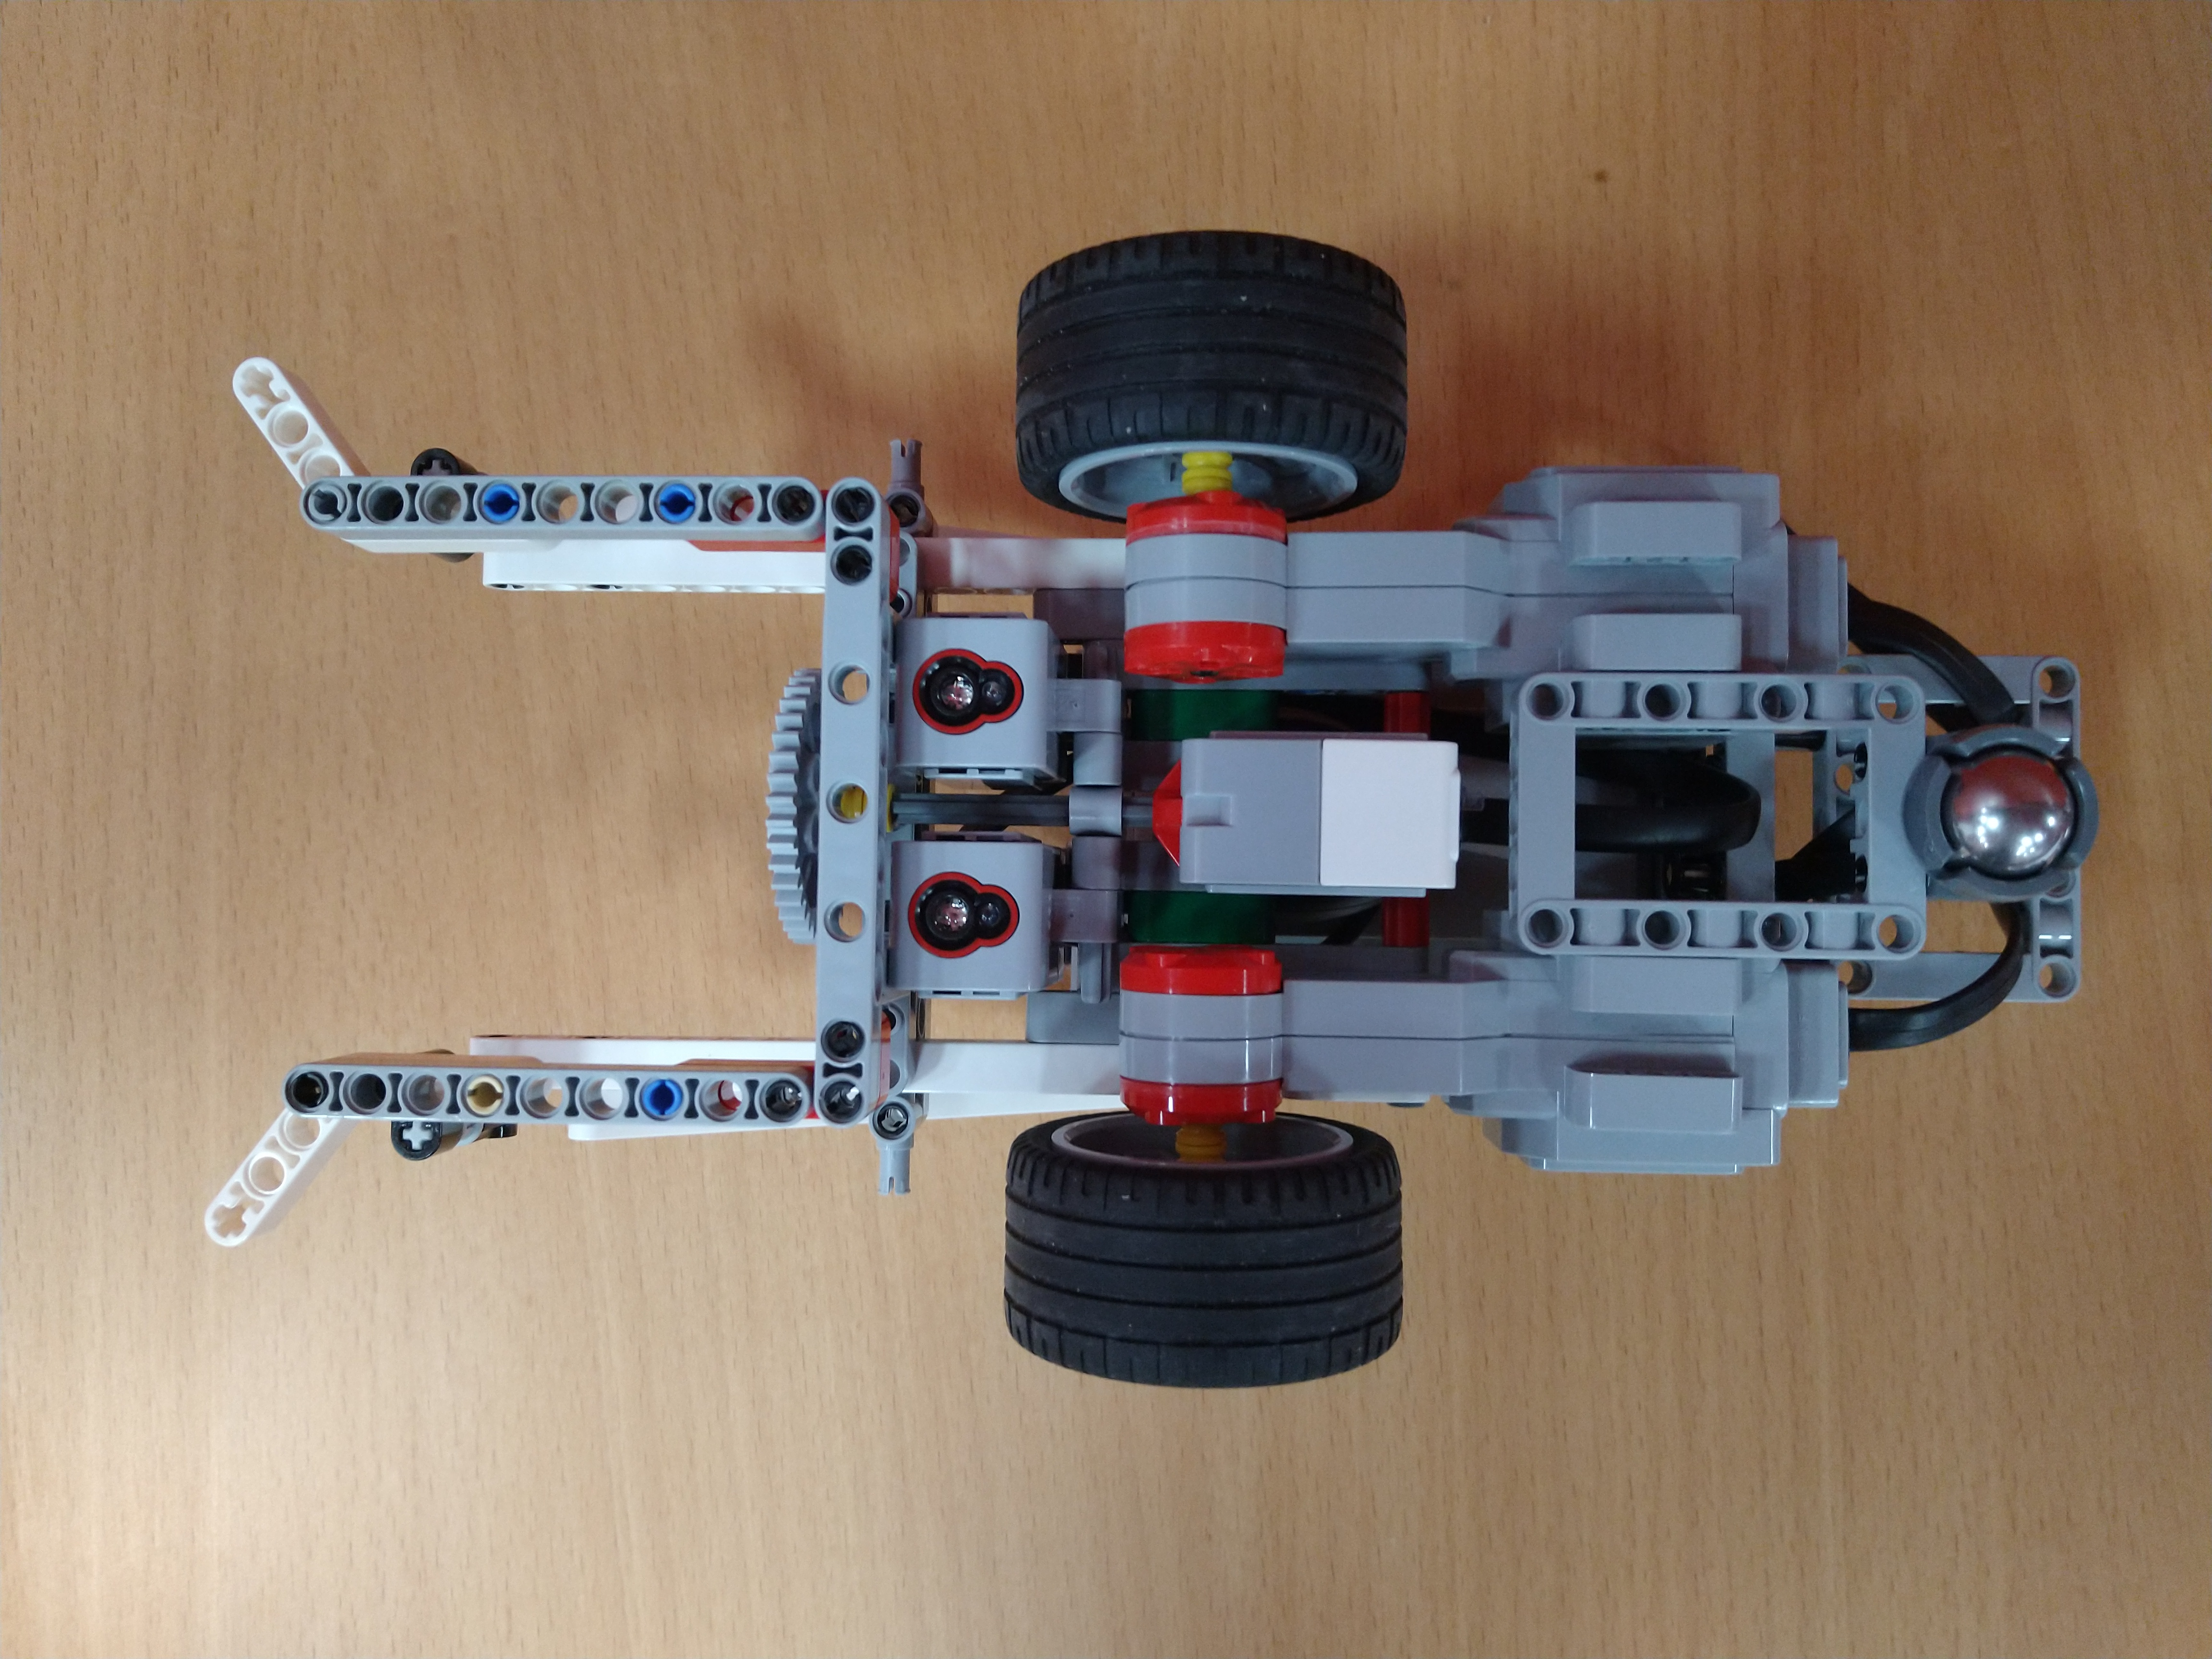
\includegraphics[width=0.8\linewidth]{images/bottom.jpg}
	\caption{images/Bottom}%
	\label{fig:images/bottom}
\end{figure}

To sense the map the color sensors are placed far enough apart to allow a line between them.
This is to ensure that the root will not jitter and constantly correct its course while
following the map.

The sensors can be seen on figure \ref{fig:images/bottom}.


To sense the can, a pressure sensor is mounted in the cage of the robot, as can be seen in figure
\ref{fig:images/bottom}.


\begin{itemize}
	\item Dependent on odometry for placing cans
	\item Cannot sense cans at a distance
	\item No good way of recovering if lost
\end{itemize}

	
\end{document}
